\section{Results and Analysis}

\subsection{Quantitative Results}

The final results for each model are presented below:

\begin{table}[htbp]
    \caption{Quantitative results of the models on the train, validation and test set.}
    \begin{center}
        \resizebox{0.9\linewidth}{!}{
            \begin{tabular}{|c|c|c|c|c|c|}
                \hline
                \textbf{Model}    & \textbf{Train Loss} & \textbf{Val Loss} & \textbf{Val Accuracy} & \textbf{Test F1-Score} & \textbf{Epochs} \\
                \hline
                Guessing Baseline & -                   & -                 & -                     & 0.14105                & -               \\
                \hline
                Custom CNN        & 0.2897              & 0.3034            & 0.9042                & 0.92695                & 64              \\
                \hline
                Pre-trained CNN   & \textbf{0.0532}     & \textbf{0.1467}   & \textbf{0.9537}       & 0.96095                & 30              \\
                \hline
                Pre-trained ViT   & 0.1438              & 0.2089            & 0.9379                & 0.96725                & 29              \\
                \hline
                \textbf{Ensemble} & -                   & -                 & -                     & \textbf{0.97103}       & -               \\
                \hline
            \end{tabular}
            \label{tab:results}
        }
    \end{center}
\end{table}

Table~\ref{tab:results} shows the performance of each model on the validation and the test set. The \textbf{custom CNN} achieved a validation accuracy of \textbf{90.42\%} and a test F1-score of \textbf{0.92695}. The \textbf{pre-trained CNN} (ResNet-18) outperformed the custom CNN with a validation accuracy of \textbf{95.37\%} and a test F1-score of \textbf{0.96095}. The \textbf{pre-trained ViT} achieved a validation accuracy of \textbf{93.79\%} and a test F1-score of \textbf{0.96725}. The \textbf{ensemble}, which combines the predictions of all three models, achieved the highest test F1-score of \textbf{0.97103}. Since the \textbf{guessing baseline} and the \textbf{ensemble} are not trained models, the training and validation losses are not applicable.

\subsection{Qualitative Results}

Since the labels for the test set are not available, the qualitative results are based on the validation set to get an idea of the performance of the models. The confusion matrices of the custom CNN, pre-trained CNN and pre-trained ViT models on the validation set are shown below:

\begin{figure}[htbp]
    \centerline{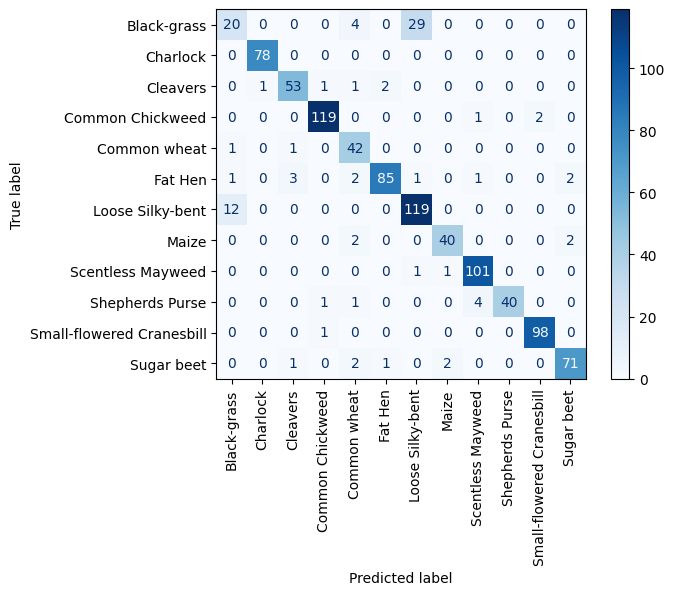
\includegraphics[width=0.9\linewidth]{../../resources/custom_cnn/confusion.png}}
    \caption{Confusion Matrix (custom CNN)}
    \label{fig:confusion-matrix-custom-cnn}
\end{figure}

Fig.~\ref{fig:confusion-matrix-custom-cnn} shows the confusion matrix of the custom CNN on the validation set. The rows represent the true classes, while the columns represent the predicted classes. The diagonal elements represent the number of correct predictions for each class, while the off-diagonal elements represent the misclassifications. While there are some misclassifications without a clear pattern, the model clearly struggles to distinguish between ``Loose Silky-bent'' and ``Black-grass''.

\begin{figure}[htbp]
    \centerline{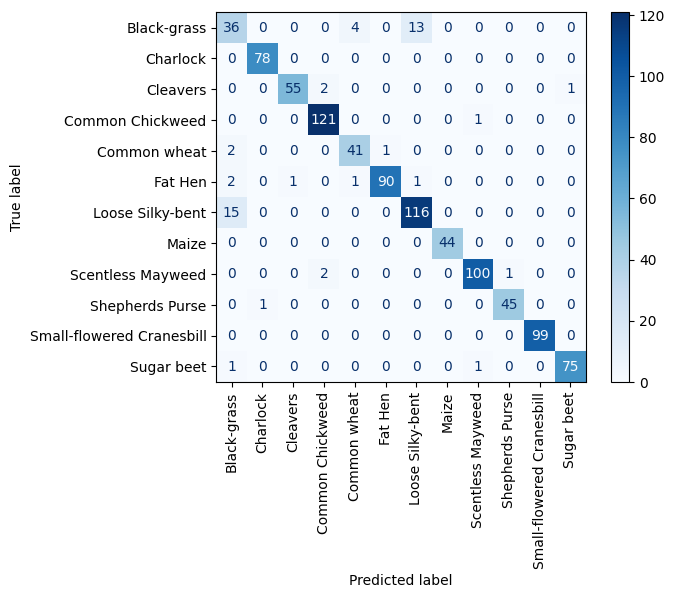
\includegraphics[width=0.9\linewidth]{../../resources/resnet/confusion.png}}
    \caption{Confusion Matrix (pre-trained CNN)}
    \label{fig:confusion-matrix-pretrained-cnn}
\end{figure}

Similar to the custom CNN, Fig.~\ref{fig:confusion-matrix-pretrained-cnn} shows the confusion matrix of the pre-trained CNN on the validation set. The model shows the same difficulty in distinguishing between ``Loose Silky-bent'' and ``Black-grass''.

\begin{figure}[htbp]
    \centerline{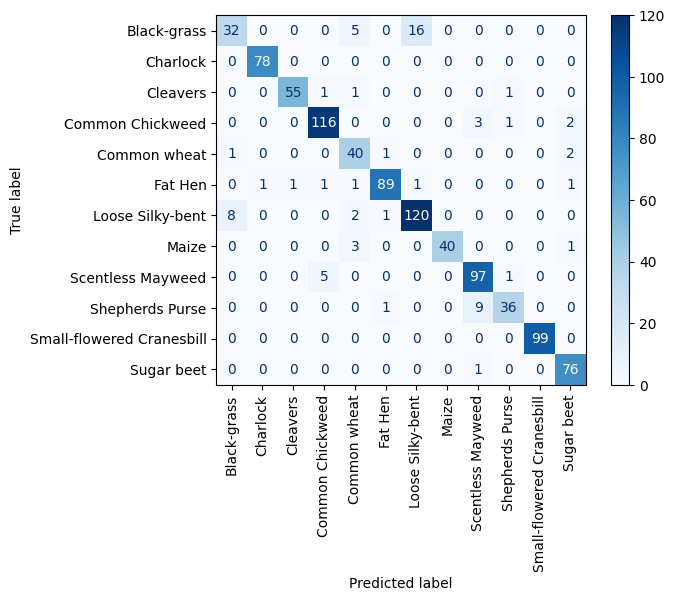
\includegraphics[width=0.9\linewidth]{../../resources/vit/confusion.png}}
    \caption{Confusion Matrix (pre-trained ViT)}
    \label{fig:confusion-matrix-pretrained-vit}
\end{figure}

Although the pre-trained ViT model takes a different approach, Fig.~\ref{fig:confusion-matrix-pretrained-vit} shows that it also struggles with the same pair of classes ``Loose Silky-bent'' and ``Black-grass''.

\subsection{Comparative Analysis}

The results show that the ensemble model outperforms the individual models, achieving the highest test F1-score of \textbf{0.97103}. The pre-trained ViT model achieved the highest individual test F1-score of \textbf{0.96725}, followed by the pre-trained CNN with a test F1-score of \textbf{0.96095}. The custom CNN achieved a test F1-score of \textbf{0.92695}, demonstrating competitive performance despite being trained from scratch.

Since real-time inference is not required for this task, the computational cost of the models is not a primary concern. However, the custom CNN is the lightest model with approximately \textbf{2 million} parameters, making it computationally efficient. The pre-trained CNN has approximately \textbf{11 million} parameters, while the pre-trained ViT has approximately \textbf{85 million} parameters, making it the most computationally expensive model.

\subsection{Interpretability Measures}

The Pytorch-Grad-CAM library~\cite{jacobgilpytorchcam} by Jacob Gildenblat was used to generate class activation maps (CAMs) for the custom CNN, pre-trained CNN and pre-trained ViT models. CAMs provide insight into the regions of the image that the model focuses on when making predictions and can help explain the decision-making process of the model. The library was installed with the following command:

\begin{minipage}{0.9\linewidth}\begin{lstlisting}[language={},caption={Install Pytorch-Grad-CAM library.},label={lst:install-grad-cam}]
pip install grad-cam
\end{lstlisting}\end{minipage}

The simplified code snippet below shows how to generate CAMs for a given image using the custom CNN model:

\begin{minipage}{0.9\linewidth}\begin{lstlisting}[caption={Generate CAMs using Pytorch-Grad-CAM.},label={lst:grad-cam}]
from pytorch_grad_cam import GradCAM
from pytorch_grad_cam.utils.image import show_cam_on_image
from pytorch_grad_cam.utils.model_targets import ClassifierOutputTarget

with GradCAM(
        model=model,
        target_layers=target_layers,
     ) as cam:
    grayscale_cam = cam(
                        input_tensor=image.unsqueeze(0),
                        targets=targets,
                    )
    grayscale_cam = grayscale_cam[0, :]
    visualization = show_cam_on_image(
                        rgb_img,
                        grayscale_cam,
                        use_rgb=True,
                    )
\end{lstlisting}\end{minipage}

The following figures show Grad-CAM visualizations for the last two layers of the custom CNN, pre-trained CNN and pre-trained ViT models:

\begin{figure}[htbp]
    \centerline{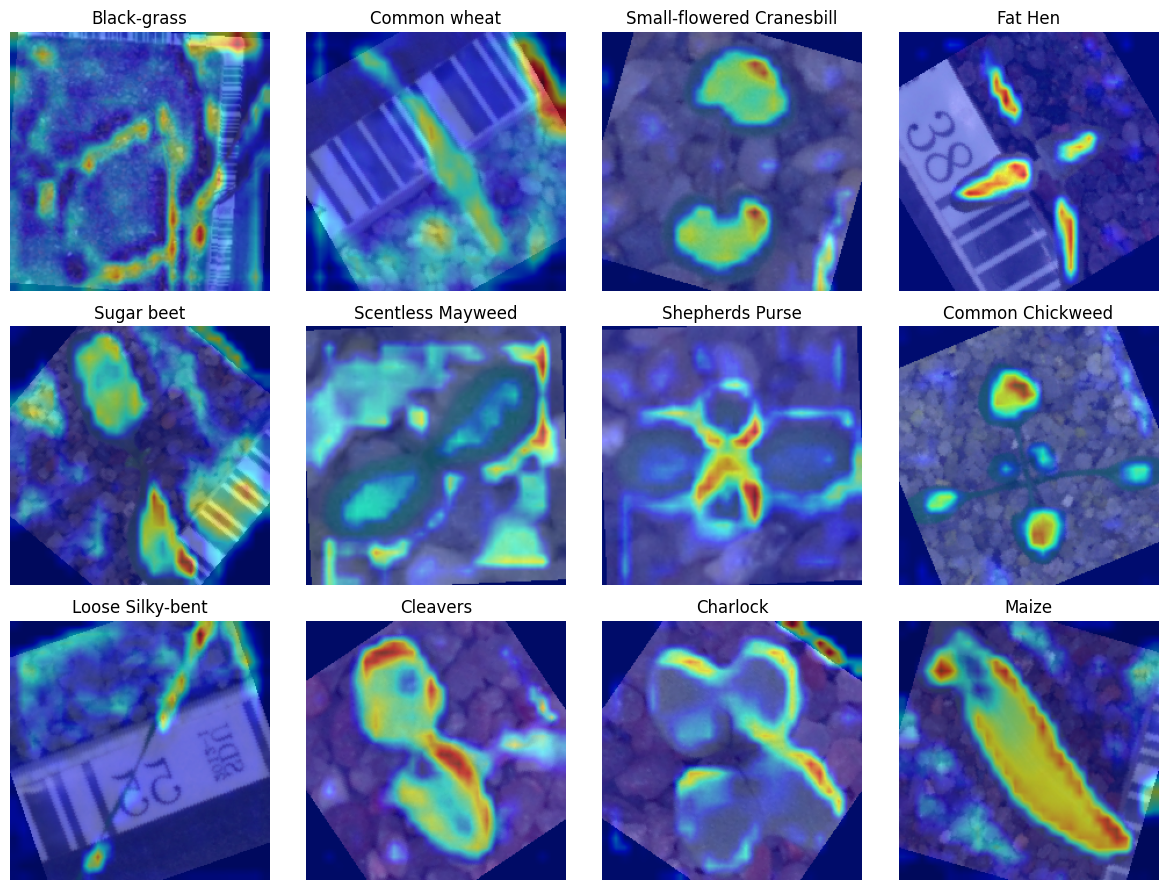
\includegraphics[width=0.9\linewidth]{../../resources/custom_cnn/grad_cam.png}}
    \caption{Grad-CAM (custom CNN)}
    \label{fig:grad-cam-custom-cnn}
\end{figure}

\begin{figure}[htbp]
    \centerline{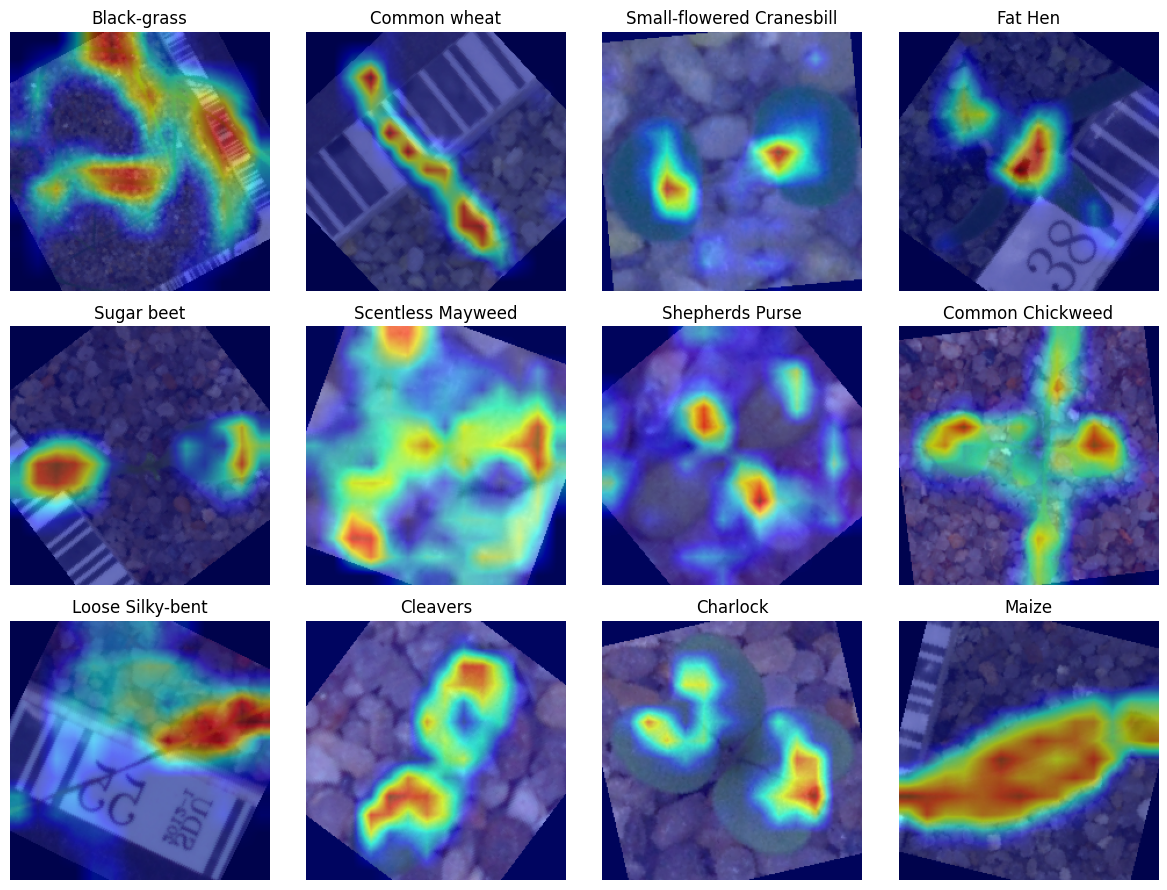
\includegraphics[width=0.9\linewidth]{../../resources/resnet/grad_cam.png}}
    \caption{Grad-CAM (pre-trained CNN)}
    \label{fig:grad-cam-pretrained-cnn}
\end{figure}

\begin{figure}[htbp]
    \centerline{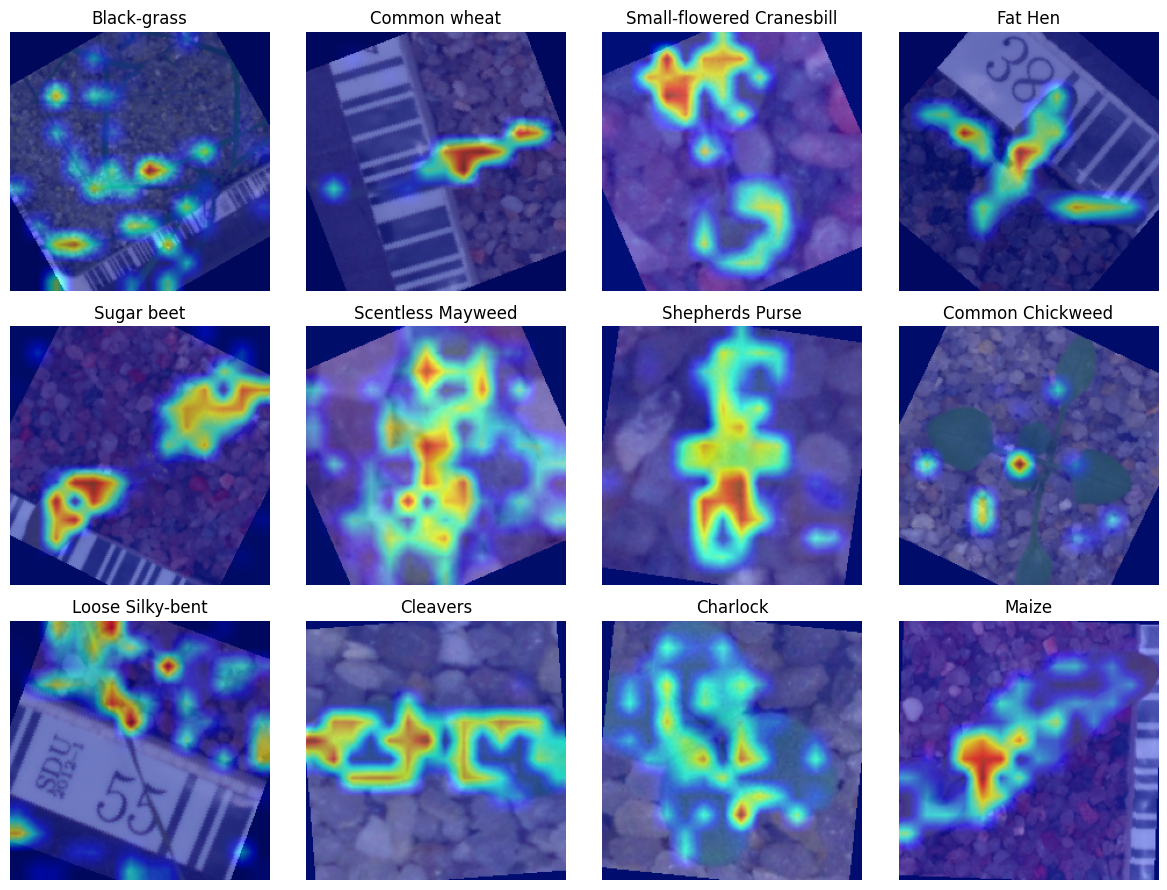
\includegraphics[width=0.9\linewidth]{../../resources/vit/grad_cam.png}}
    \caption{Grad-CAM (pre-trained ViT)}
    \label{fig:grad-cam-pretrained-vit}
\end{figure}

The Fig.~\ref{fig:grad-cam-custom-cnn}, Fig.~\ref{fig:grad-cam-pretrained-cnn} and Fig.~\ref{fig:grad-cam-pretrained-vit} show the Grad-CAM visualizations for the custom CNN, pre-trained CNN and pre-trained ViT models. The visualizations highlight the regions of the image that the model focuses on when making predictions. The Grad-CAM visualizations provide insight into the decision-making process of the models and help to interpret their predictions.

For some classes, such as ``Small-flowered Cranesbill'', ``Fat Hen'', ``Common Chickweed'', ``Cleavers'' and ``Maize'', the custom CNN clearly focuses on parts of the plants that a human would use to distinguish between the classes. For these species, the focus is on the leaves. For classes like ``Black-grass'', ``Common wheat'', ``Sugar beet'', ``Scentsless Mayweed'' and ``Loose Silky-bent'' the CNN focuses on what appears to be the soil or the background. One could argue that the model has difficulty distiguishing between the plants and the background and focuses on *noise* in the images.

In comparison, both pre-trained architectures, the CNN and the ViT, focus more on the plants themselves. But even for ``Black-grass'', ``Scentsless Mayweed'' and ``Loose Silky-bent'' the models do not seem to focus on the plants alone. The visualizations of the areas of interest are smoother for the CNN compared to the ViT, which looks more *blocky*. This is due to the different architectures and the way the models process the images as the ViT divides the image into patches and processes them separately, therefore the patches are more visible in the Grad-CAM visualizations for the ViT. For a human observer the Grad-CAM visualizations can help understand how the models make their predictions and what features they focus on, the custom CNN seems to produce the most resonable visualizations and focus on understandable features.